\section{Execution and deployment.}\label{sec:network}
In the context of \evlbi\ the software correlator can be executed in
two different operational modes that are: \emph{batch-execution} and
\emph{real-time}. Grids have a long history in running batch jobs and
grid-middleware is now doing a good job on this task. The execution of
real-time applications is much more complex; grid infrastructure and
middleware have to provide guarantees on the Quality of the Service to
insure successful execution of the job. Quality of Service management
in grids is still evolving rapidly. To experiment with these aspects
we are running \scarie\ on a research grid called DAS-3 and its
manageable network called StarPlane.

\subsection{Real-time and quality of service}
The term \emph{real-time} has many definitions in the computer science
community, in this paper we will consider that a \emph{real-time}
computation is a computation in which: \emph{the amount of buffering
  for an infinitely long experiment will only require a finite amount
  of buffers}. This is a formal way to define a process in which the
incoming data are "consumed" by the computation as fast as they are
generated. This definition also implies that once the application is
started the allocated "space" on the resources will be maintained
during the complete execution.

The main resources \scarie\ is using are: the network bandwidth, the
computation resource and the disk-space. Sharing of the computational
resource is now a well understood process and most of the time it is
part of the execution service that allocates the requested resources
and if all resources are acquired, it deploys and executes the
application.
\begin{comment}
\begin{figure}
  \centering
  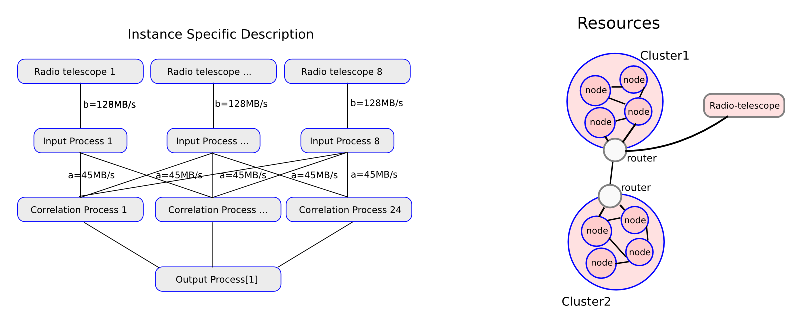
\includegraphics[width=\textwidth]
    {img/mapping.eps}
    \caption{Left: An specific instaInce of an experiment. Right: The
      resource set. Resource allocation and application scheduling
      have to map the left side to the resources. }
  \label{fig:mapping}
\end{figure}
\end{comment}
The simplest way to offer guaranteed service over a shared resource
can be done by restricting the access to only one user at a time. This
approach is used in the DAS-3 grid (based on SGE) in which an
allocated node is simply unusable by other users. Same principle could
be applied to the complete grid including its networks and other
resources. A more flexible approach consists in sharing the resource
under the arbitration of a third party that will insure that each
application is using only the allocated part of the resource. This is
the case with Layer-3 QoS for networks, or the recently added
Completely Fair Scheduler (per application CPU time allocation) or per
application IO-bandwith arbitration\cite{}\marginpar{DAMIEN: TODO}. In
a very general point of view all these technologies virtualize the
resource thus they permit to build on top of a real grid a complete
isolated environment based on user requirements.

\subsection{Running \scarie on \das3 and Starplane}
Networking performance and QoS management is one of the most
challenging aspects of \scarie.  The regular Internet Layer3 IP
routing based on the best-effort policy has a great flexibility but is
often slow and unpredictable; on the other hand, we have dedicated
\textit{lightpaths} as available in \textit{lambda
  Grids}~\cite{eslea-2007}\marginpar{DAMIEN}, with their predictable
delays and throughputs offer good performances and a good basis to
offer Quality of Service. Giving end users access to dedicated
connection has been implemented in many of the current research and
education networks. The Dutch National Resarch and Education network
SURFnet is one of them.  This is used to deliver the data from the
radio-telescope to the computation center.

In \scarie\ having lighpaths between radio-telescopes and the
computation center is not sufficient to insure real-time
operation. \scarie\ also uses the network to distribute the
correlation. Therefore, a per application manageable network is then
required. The \das3\ supercomputer~\cite{das3} is composed of fives
clusters located in the Netherlands and connected by a photonic
network called StarPlane. The StarPlane project manages eight
wavelengths with the goal to build a network service that permits
\textit{an application-controlled photonic network and node-to-node
  traffic isolation}. The novelty of the StarPlane project lies in its
attempt to build a virtual network service at the lowest possible
networking layer: the photonic layer for the optical part and
ethernet-layer2 for the connection to the nodes. This permits to
improve performance and to dramatically reduces the cost (the price or
the energy) per byte transfered \cite{}\marginpar{TODO}. Another
property of StarPlane is that the photonic lightpath can dynamically
be reorganized to match the requirements of the user-application. By
using StarPlane, a complete virtual network over distributed cluster
sites can be build on demand. The lighpaths can also be re-organized
at run-time if the network load changes. For \scarie this allows us to
distribute the workload over several cluster locations while taking
profit of the high-bandwidth with a relative good QoS control over the
complete network domain.

\subsection{Benchmarks on DAS-3}
\scarie~ and StarPlane have parallel roadmaps. Hence the complete
approach cannot be tested yet. We have conducted correlator
performance tests using \das3. The current software correlator is
currently able to perform a 4x128Mbps\marginpar{NGHK: CHECK}
experiment at 20\% of the real-time speed using a total of 16 (quad
core 2.0Ghz cpu) nodes.

In parallel with the benchmarks of the correlator, we are also testing
the capabilities of StarPlane to do high performance traffic isolation
that is needed for real-time correlation. At the time of writing
StarPlane has implemented the service that allows a program to build
and allocate a lighpath between two clusters on demand. We tested this
feature by running two client-server applications transmitting data
between clusters.

The network traffic of the two applications is depicted in
Figure~\ref{fig:timing}.  At the start of the application, a request
for lighpath allocation is issued (arrow 1). After a while the
throughput drops because the second application starts sending data as
well (arrow 2).  As long as the lighpath is not ready (photonic
switching takes 10 minutes) the application is sending the traffic to
the default 1Gb/s ethernet route; when the lighpath is ready (arrow 3)
the traffic is rerouted to the lightpath.

\begin{figure}[ht]
  \centering
  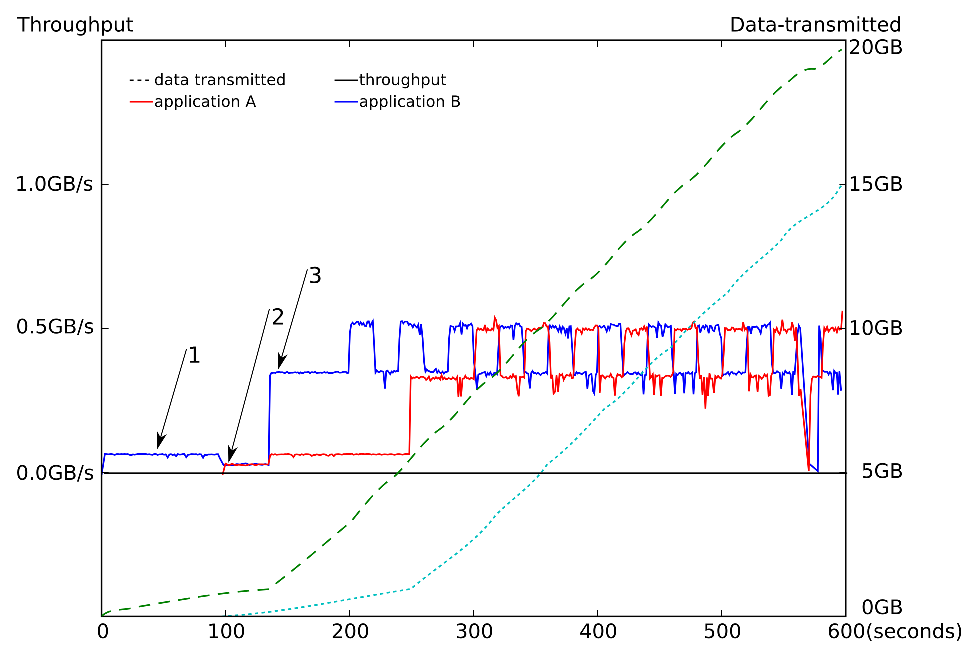
\includegraphics[width=\textwidth] {img/timing.eps}
  \caption{\label{fig:timing} Two application are started at time
    (arrow 1) and (arrow 2). The two applications have to share the
    1Gbps network bandwith. When a lighpath is allocated (arrow 3) the
    increase in performance is clearly visible.}
\end{figure} 

The results of this experiment are encouraging as they show that good
network performance can be obtained between several cluster
locations. Lighpath dynamic switching also permits to adapt the
photonic part of the network to the software correlation work load and
distribution.  Neverthless the results of this experiment also rise
questions, the secured lightpath is supposed to deliver reliably
"550MB/s" of throughput between a pair of clusters.  In
Figure~\ref{fig:timing} we can see a periodic artifact, the traffic
falling down to 300MB/s for few seconds, for which we have no
explanation. A second issue to investigate is that from time to time
the lighpath connectivity disapears entirely (e.g. at second 580). We
are currently working with Starplane team to understand and solve
these problems.


%%% Local Variables:
%%% mode: latex
%%% TeX-master: "Ingrid"
%%% End:
